% STATUS: ACTIVE -- figure-only digest, user-requested selections (2026-08-03).
%          No derivation content; each page = one requested figure (pair) with a
%          one-sentence caption.  Sources: config-3 rerun with the calibrated-grade
%          w_s prior (script test_script/scratch/plot_formB_c3_prior028.m) and the
%          S2 curved-boundary study (test_script/scratch/gainlaw_fit_cell.m).
% ======================================================
% Compile: xelatex formB_selected_figs.tex
% Path:    reference/eq17_analysis/derivation/formB_selected_figs.tex
% ======================================================

\documentclass[11pt,a4paper,fontset=none]{ctexart}

\usepackage[fleqn]{amsmath}
\usepackage{amssymb}
\setlength{\mathindent}{0pt}
\usepackage{geometry}
\geometry{margin=2.0cm}
\usepackage{graphicx}

\setlength{\parindent}{0pt}
\setlength{\parskip}{0.80em}
\linespread{1.08}

\begin{document}

\section*{Selected figures (2026-08-03)}

\begin{center}
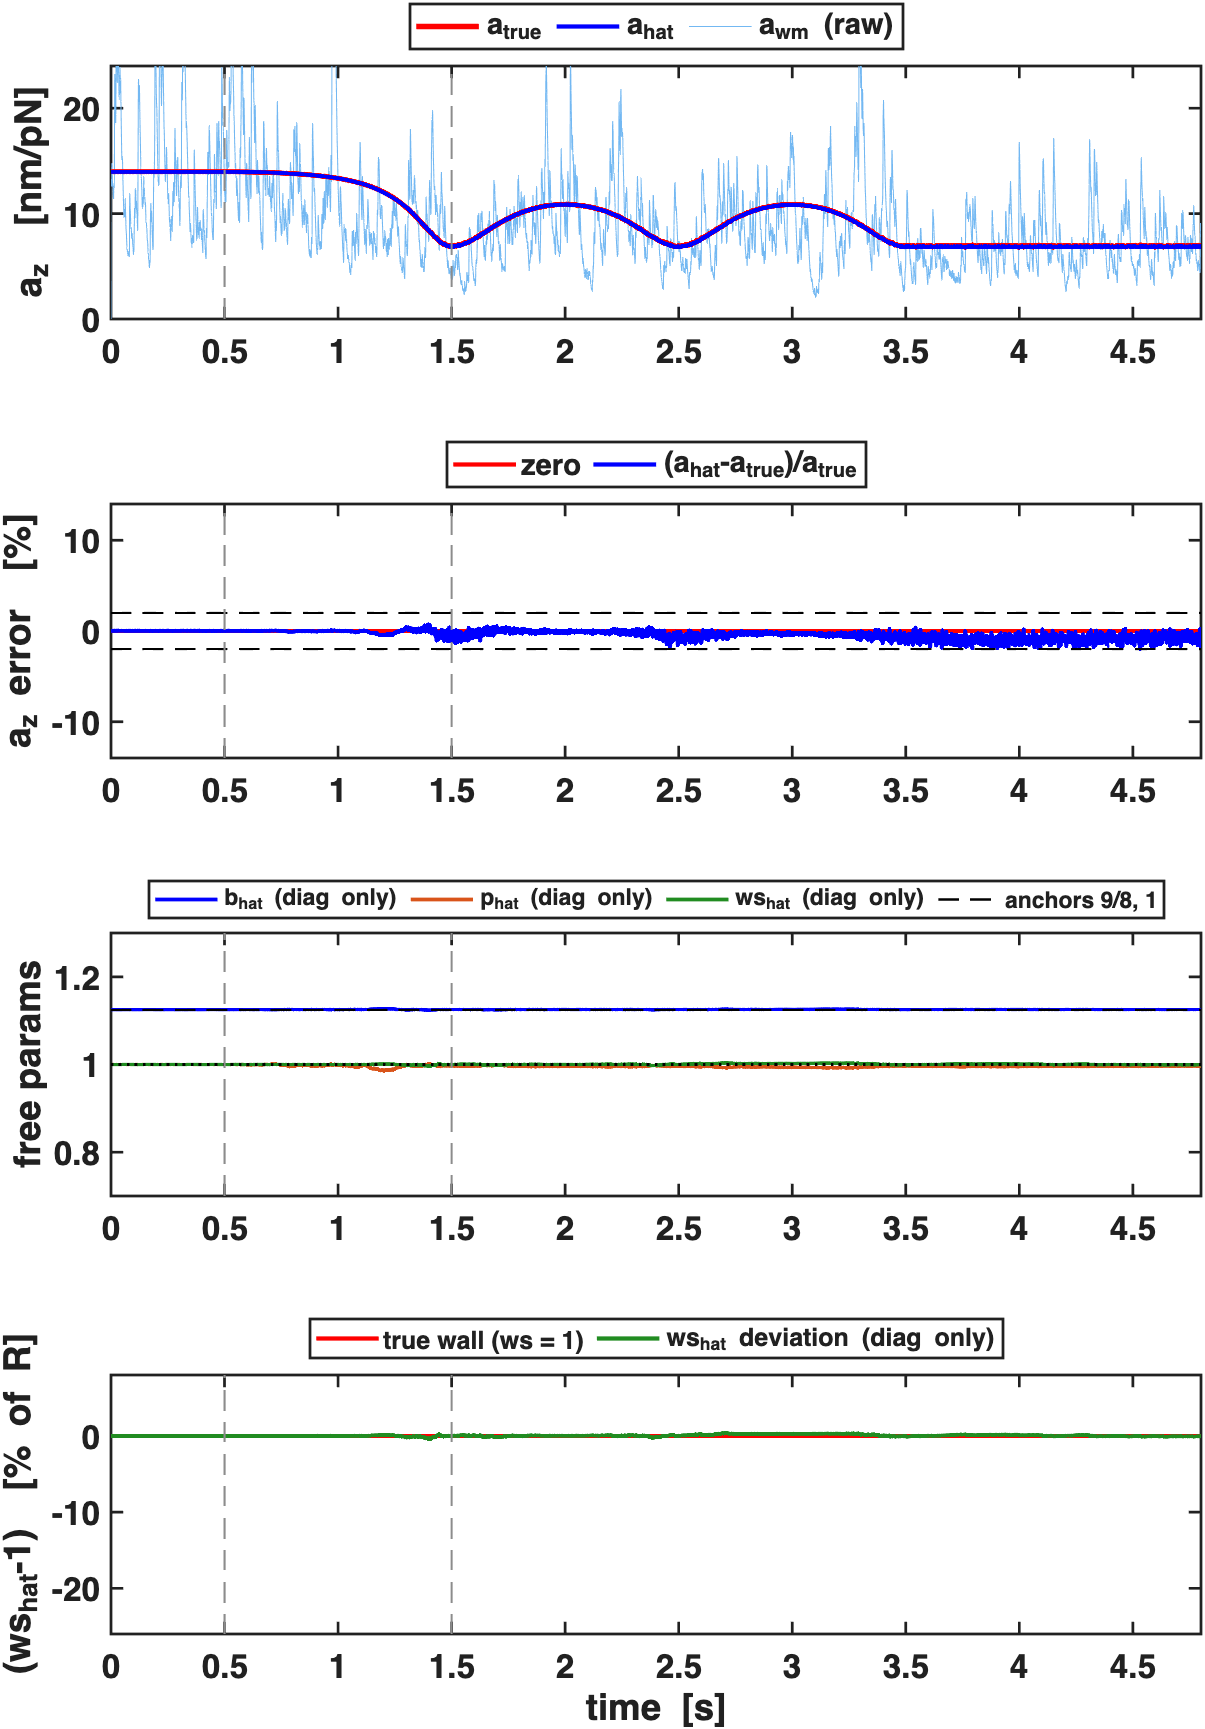
\includegraphics[width=0.49\linewidth]{figures/formB_c3_prior028_seed7.png}\hfill
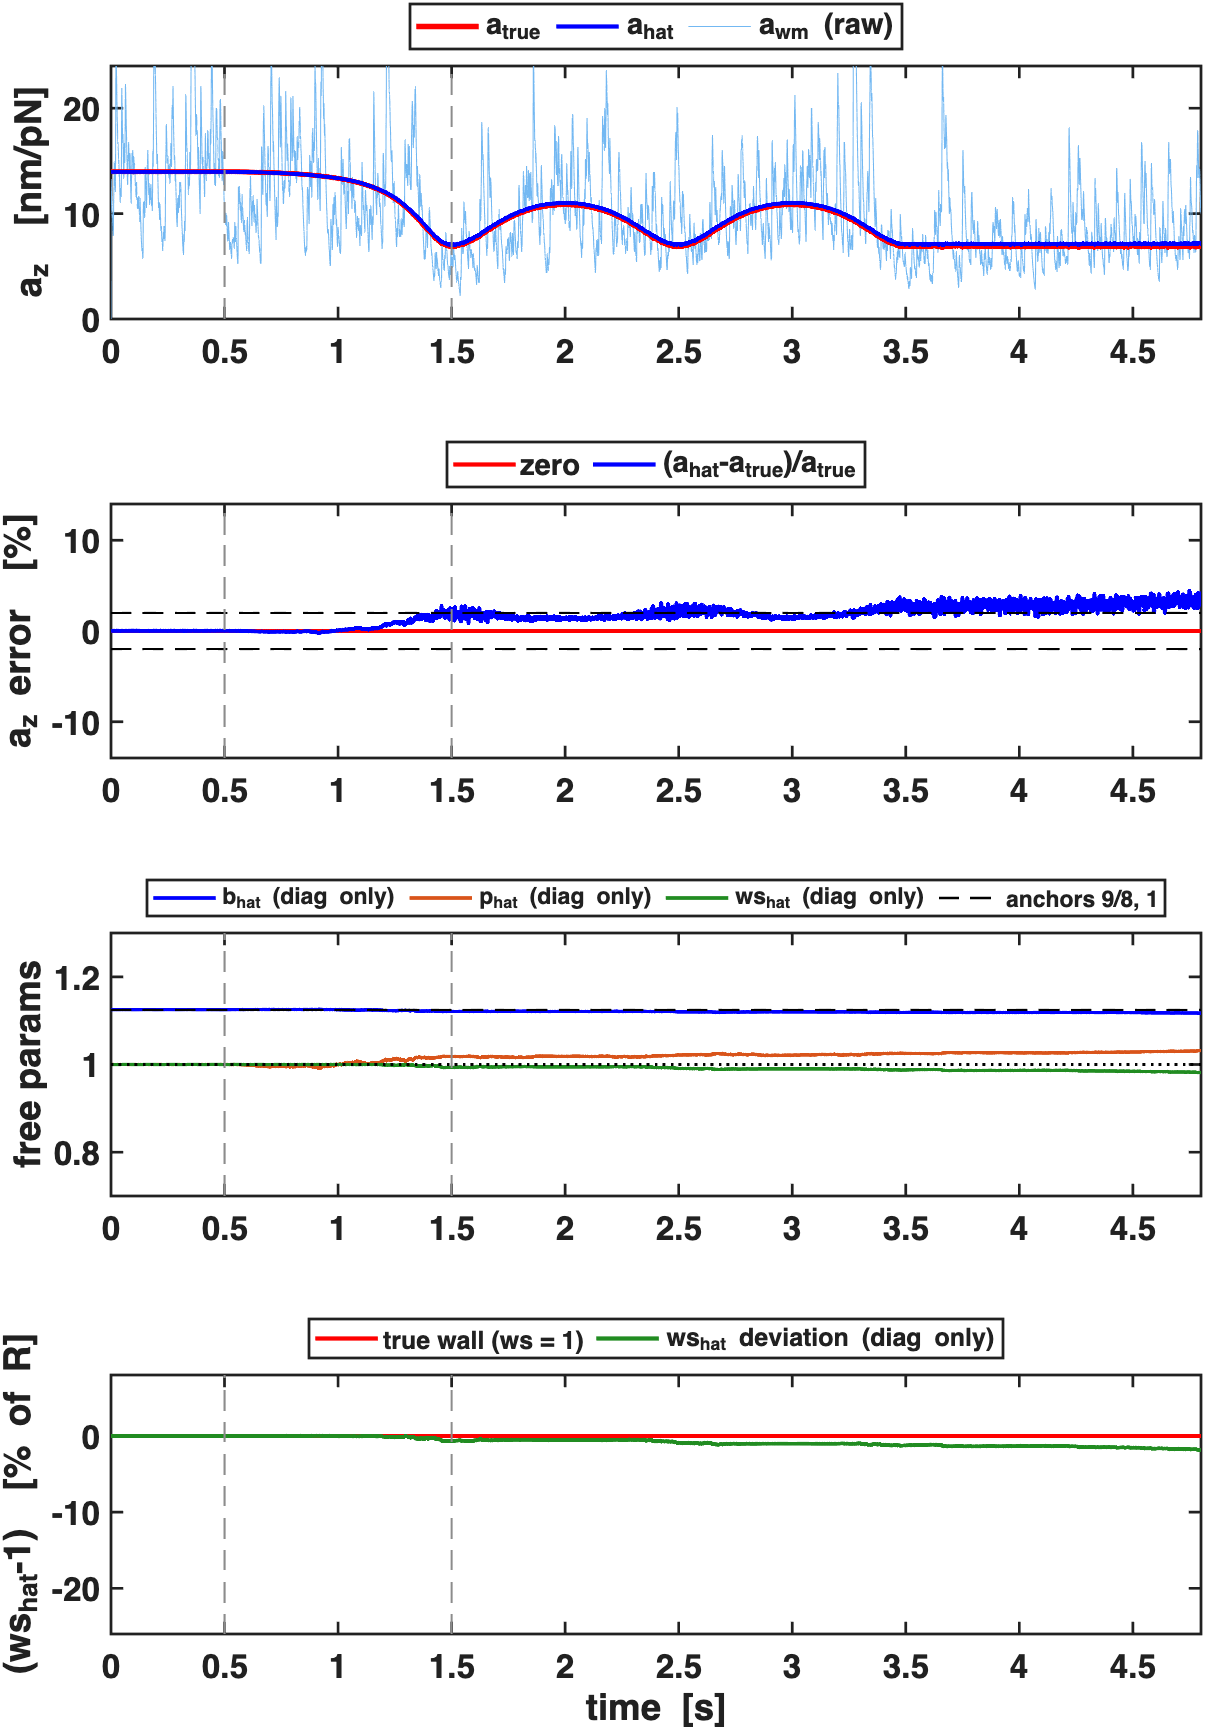
\includegraphics[width=0.49\linewidth]{figures/formB_c3_prior028_seed11.png}

Config 3 --- estimate $(b, p, w_s)$ with the calibrated-grade prior
$\sqrt{P_{w_s}}[0] = 0.028$ (house $0.111$ elsewhere unchanged): seed 7 (left)
vs seed 11 (right); the seed-11 $\hat{w}_s$ end deviation shrinks to $-1.8\,\%$
and the residual realization exits through the $b, p$ channels.
\end{center}

\clearpage

\begin{center}
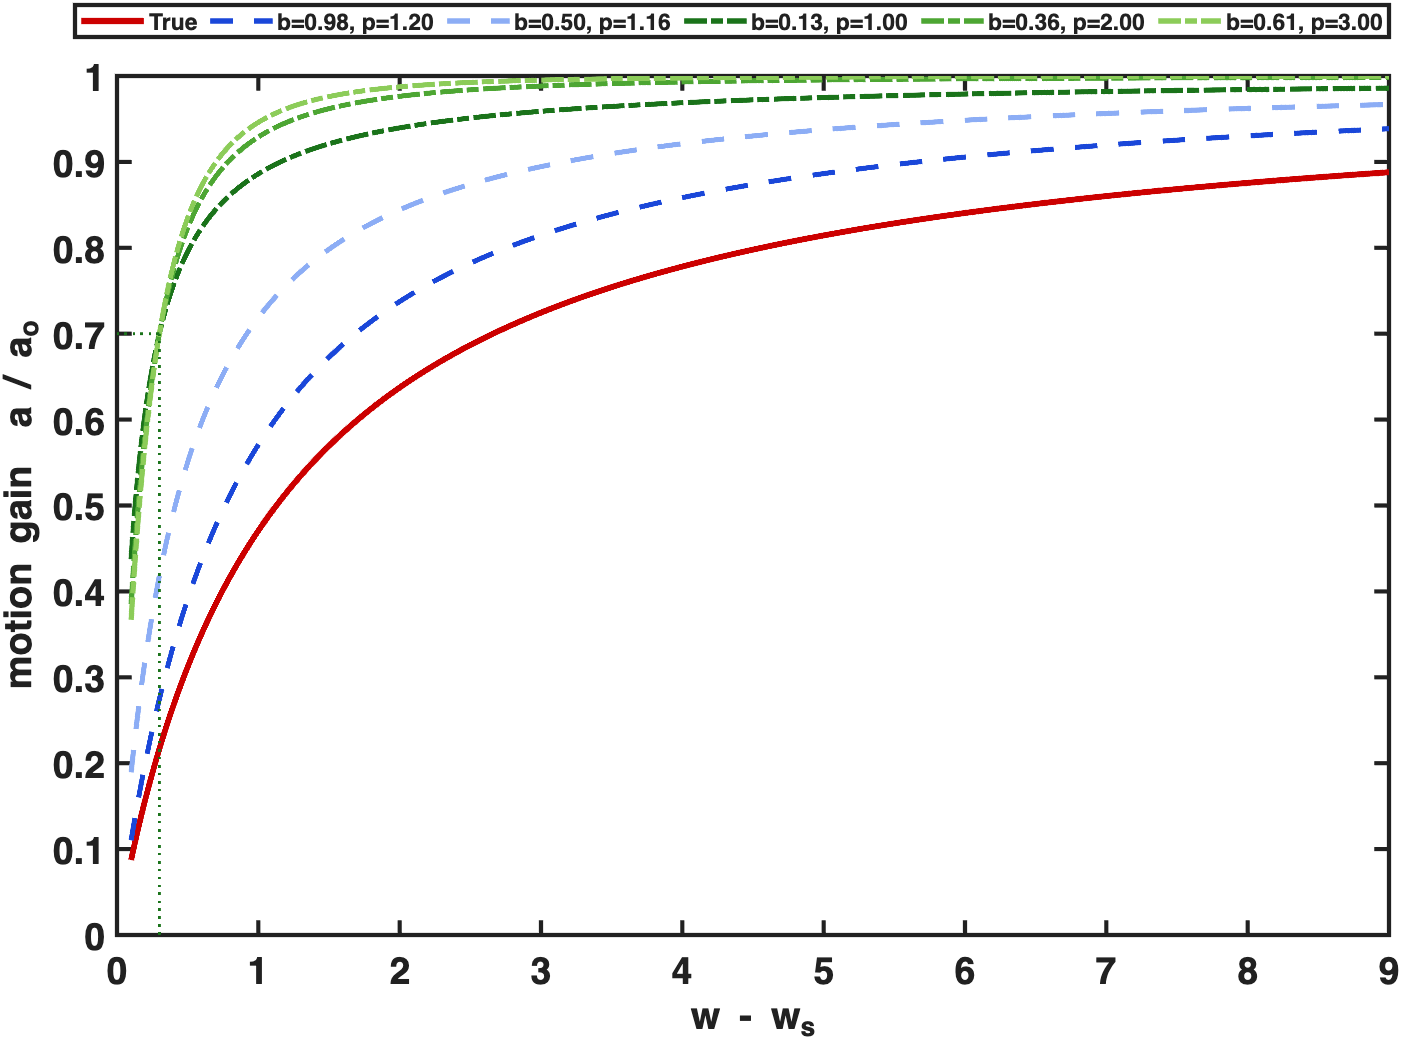
\includegraphics[width=0.85\linewidth]{figures/gainlaw_cell_fit.png}

Form B refit to two cell (two-sphere) truths against the rigid-plane truth
(red): the family absorbs boundary curvature, but the fitted $(b, p)$ leave
the plane anchors $(9/8, 1)$. The three green dash-dot curves are added by
hand: all pass through $\bar{a} = 0.70$ at a gap of $0.3\,R$ (the rigid plane
is at $0.21$ there) with the origin still on the surface, and they show the
one-parameter freedom a single point leaves --- $p$ sets the far-field decay
$1 - \bar{a} \sim g^{-p}$ and $b$ follows as $b = rG/(1-r)$,
$r = 0.3^{1/p}$.
\end{center}

\clearpage

\begin{center}
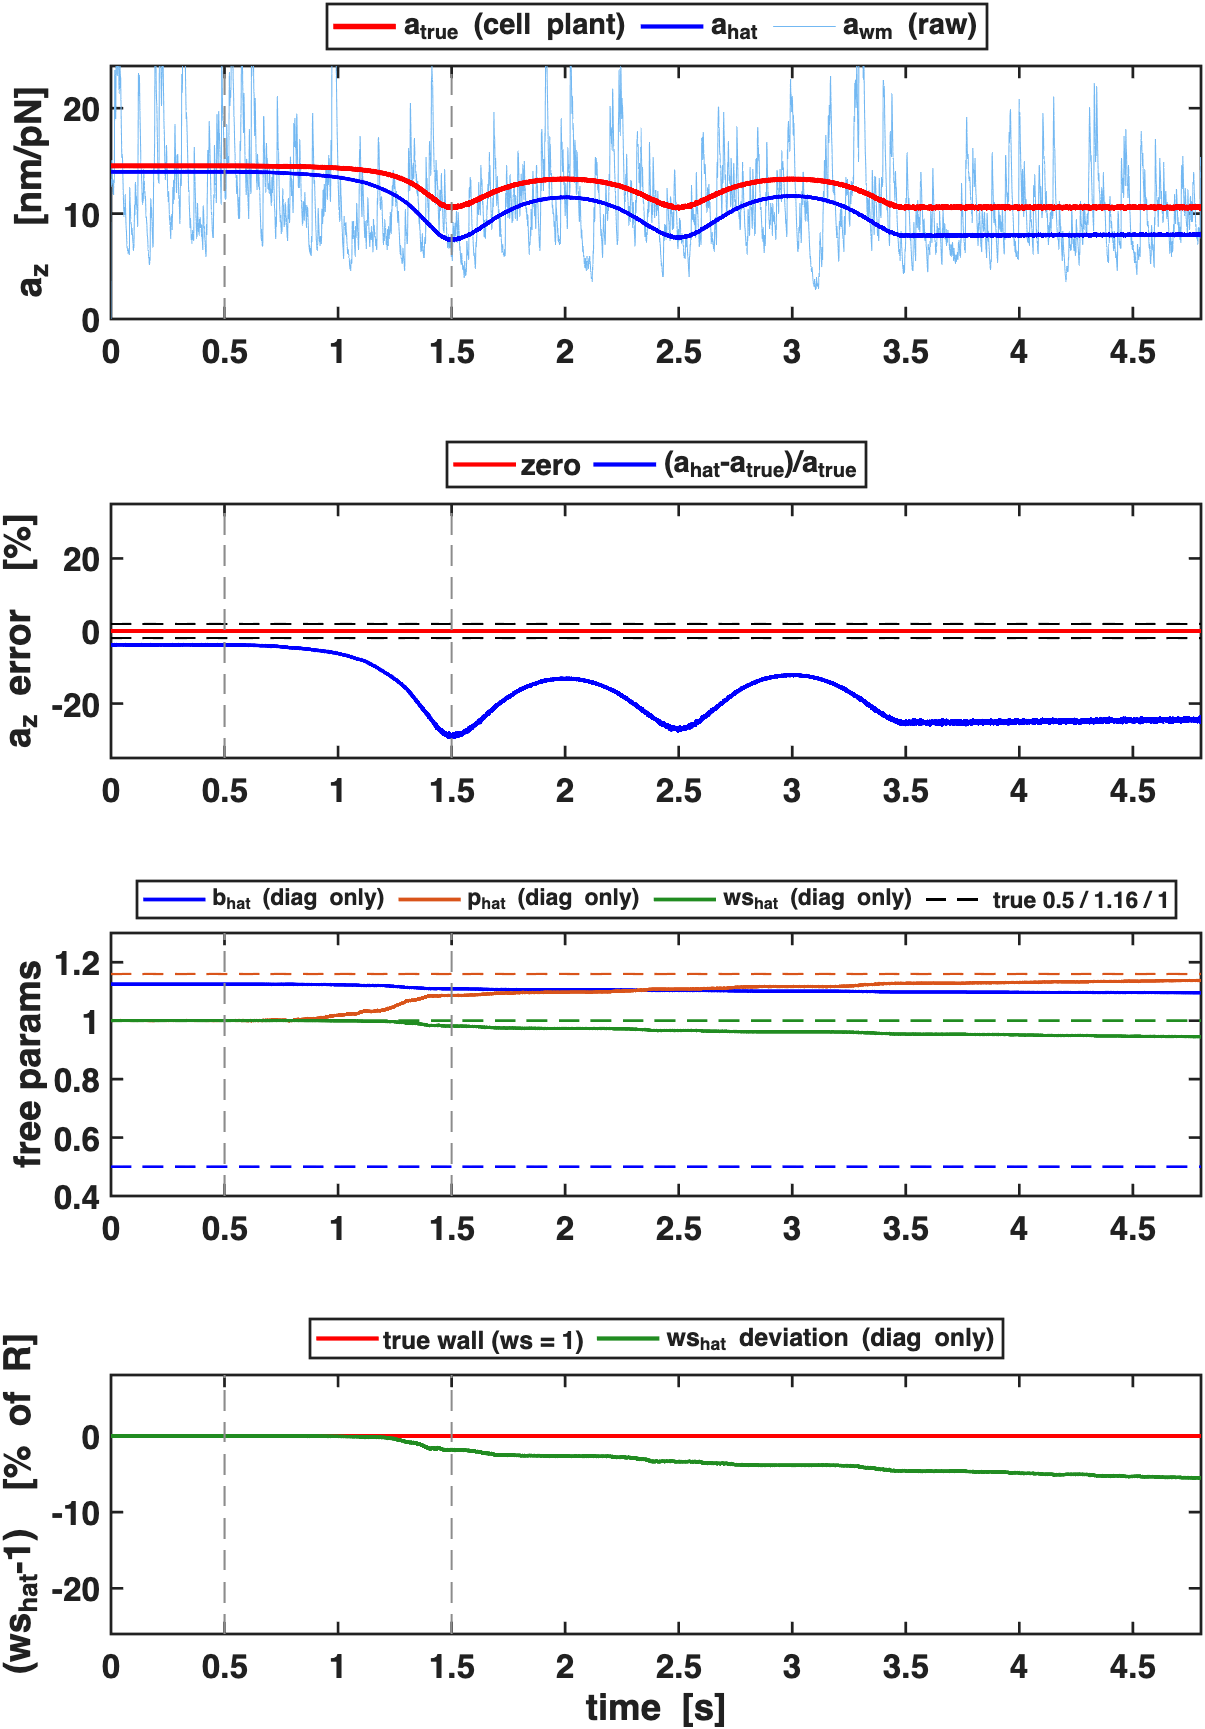
\includegraphics[width=0.49\linewidth]{figures/formB_c3_prior028_cellplant_seed7.png}\hfill
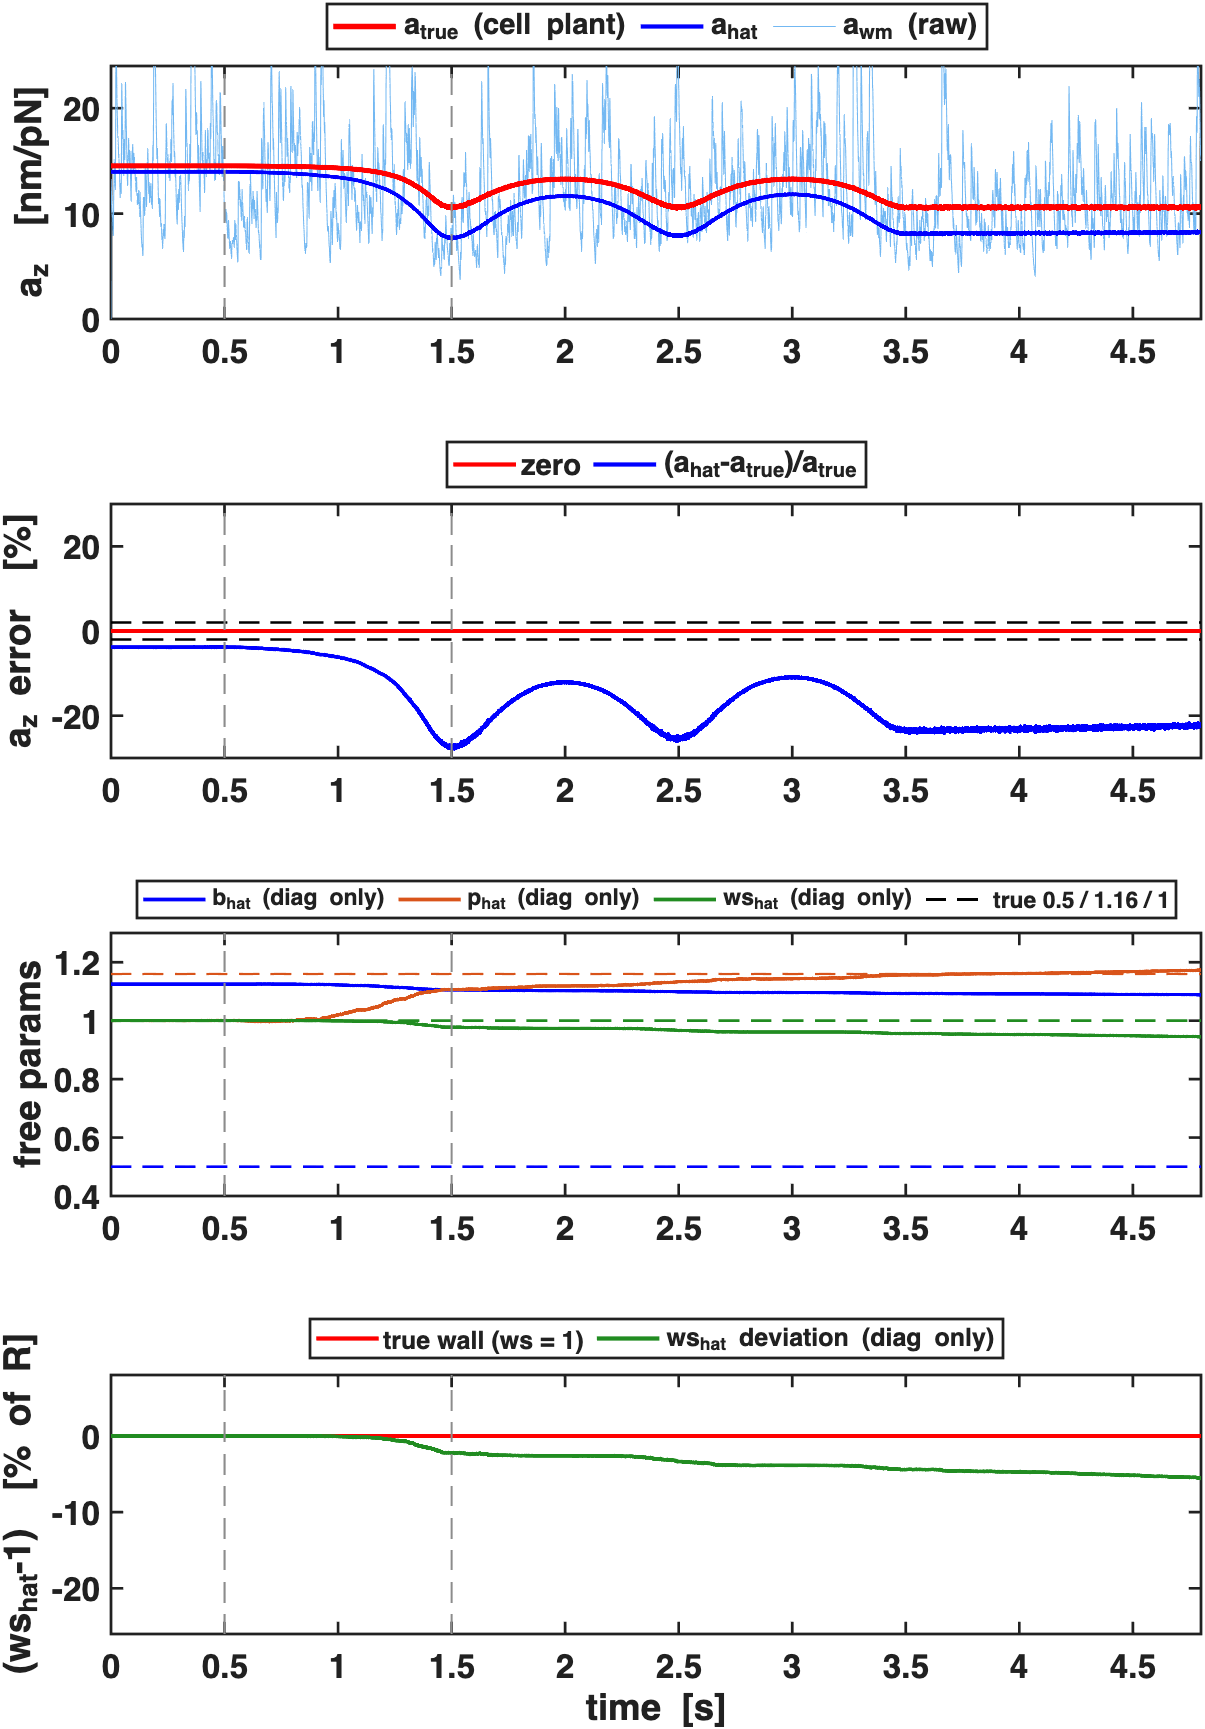
\includegraphics[width=0.49\linewidth]{figures/formB_c3_prior028_cellplant_seed11.png}

Curve-mismatch arm --- same config 3 / prior $0.028$ setup, but the TRUE $z$
curve is the cell fit $(b, p, w_s) = (0.5,\ 1.16,\ 1)$ while the controller
keeps every plane-derived prior: gain error blows up (descent peak
$\approx 28\,\%$, hold $\approx -24\,\%$), the $b, p$ traversal budgets fail by
$\sim\!50\times$, and $\hat{w}_s$ is dragged $-5.5\,\%$ against its own
$2.8\,\%$ prior --- the plane-anchored prior widths cannot absorb a boundary
this far outside the family they were derived for.
\end{center}

\clearpage

\begin{center}
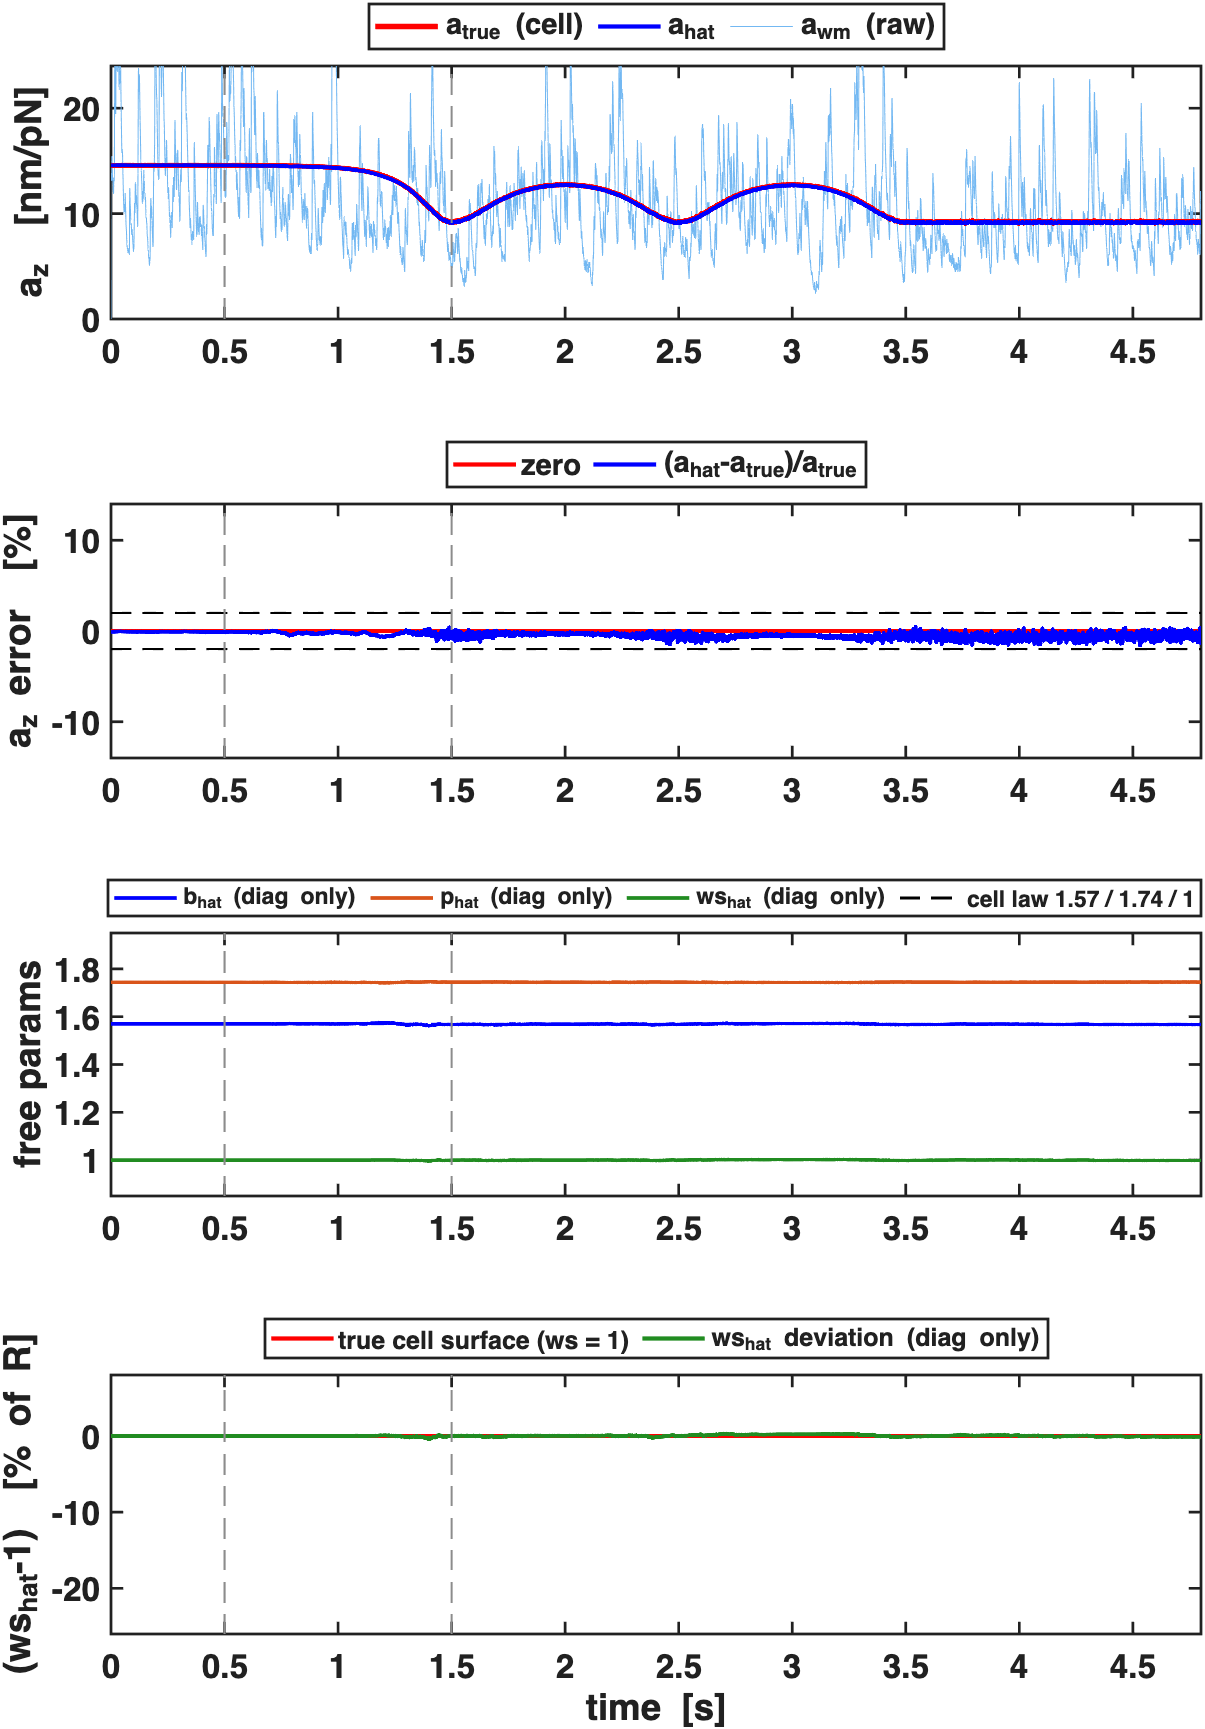
\includegraphics[width=0.49\linewidth]{figures/formB_c3_cell5_seed7.png}\hfill
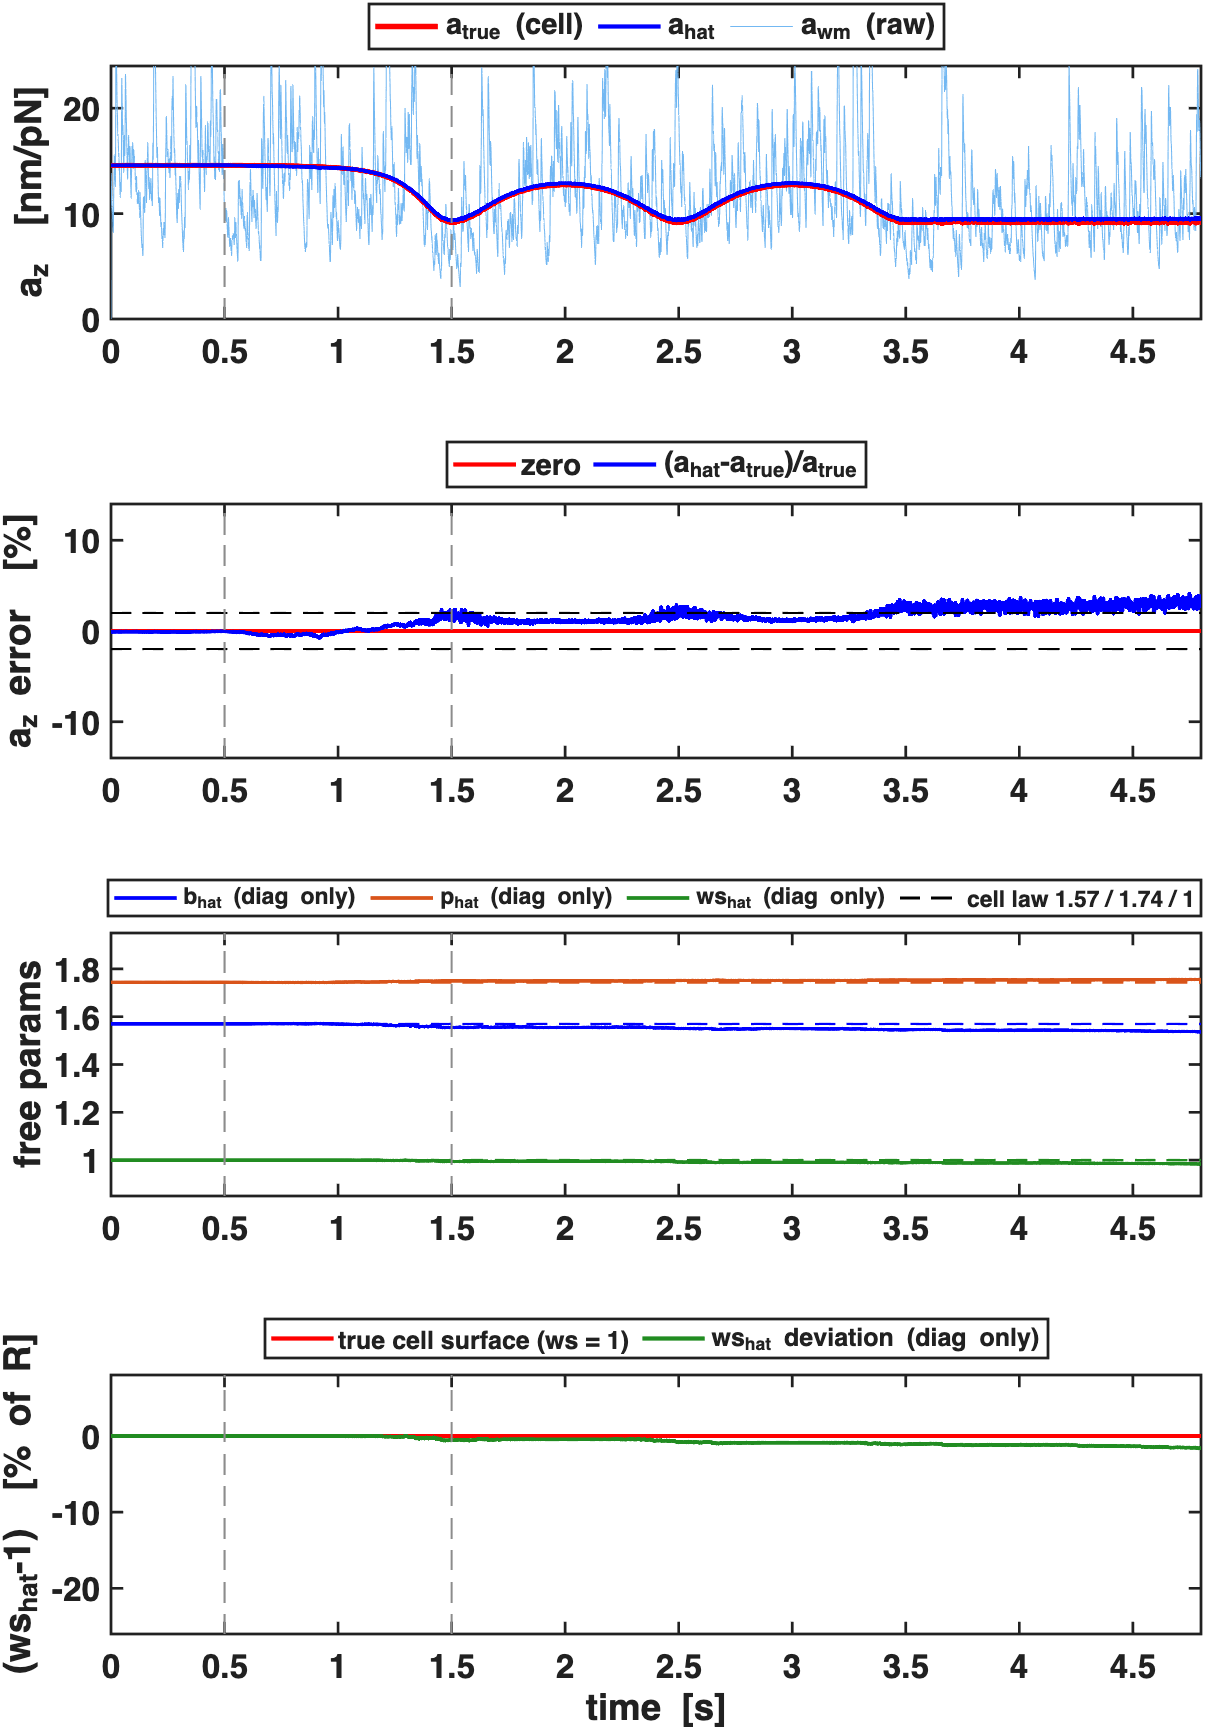
\includegraphics[width=0.49\linewidth]{figures/formB_c3_cell5_seed11.png}

Cell boundary done properly --- plant is the exact two-sphere truth for
$R_c = 5\ \mu$m and the controller carries the cell law
$(b, p, w_{s0}) = (1.570,\ 1.744,\ 0.809)$ with widths
$[0.042,\ 0.022,\ 0.015]$, fitted offline to that same published curve
(sup $0.086\,\%$): performance returns to the plane baseline
(descent $1.10/2.33\,\%$, hold $-0.61/+2.82\,\%$, $\hat{w}_s$ ending
$-0.1/-1.6\,\%$), so the difficulty was never the curvature but the anchor.
This page is the capability bound (``if we knew''), not the operating case.
\end{center}

\clearpage

\begin{center}
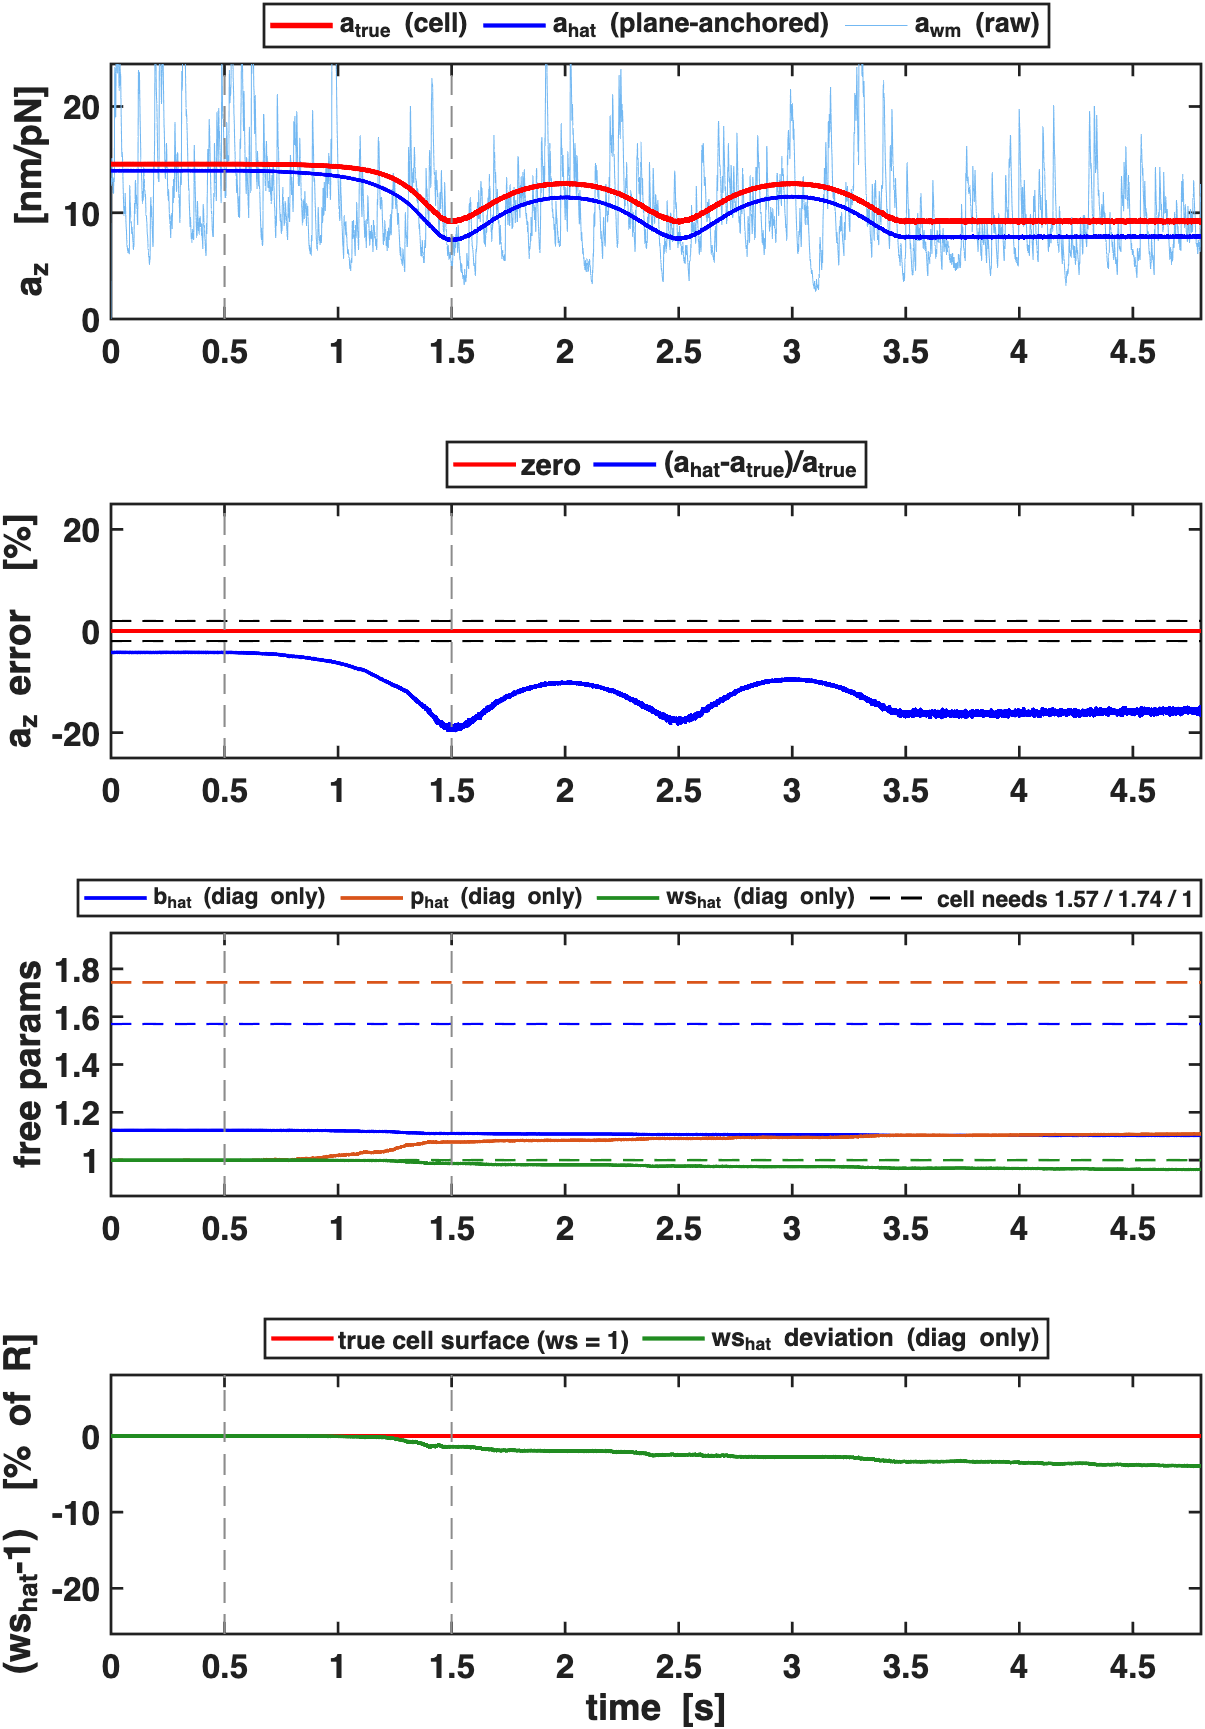
\includegraphics[width=0.49\linewidth]{figures/formB_c3_cellblind5_seed7.png}\hfill
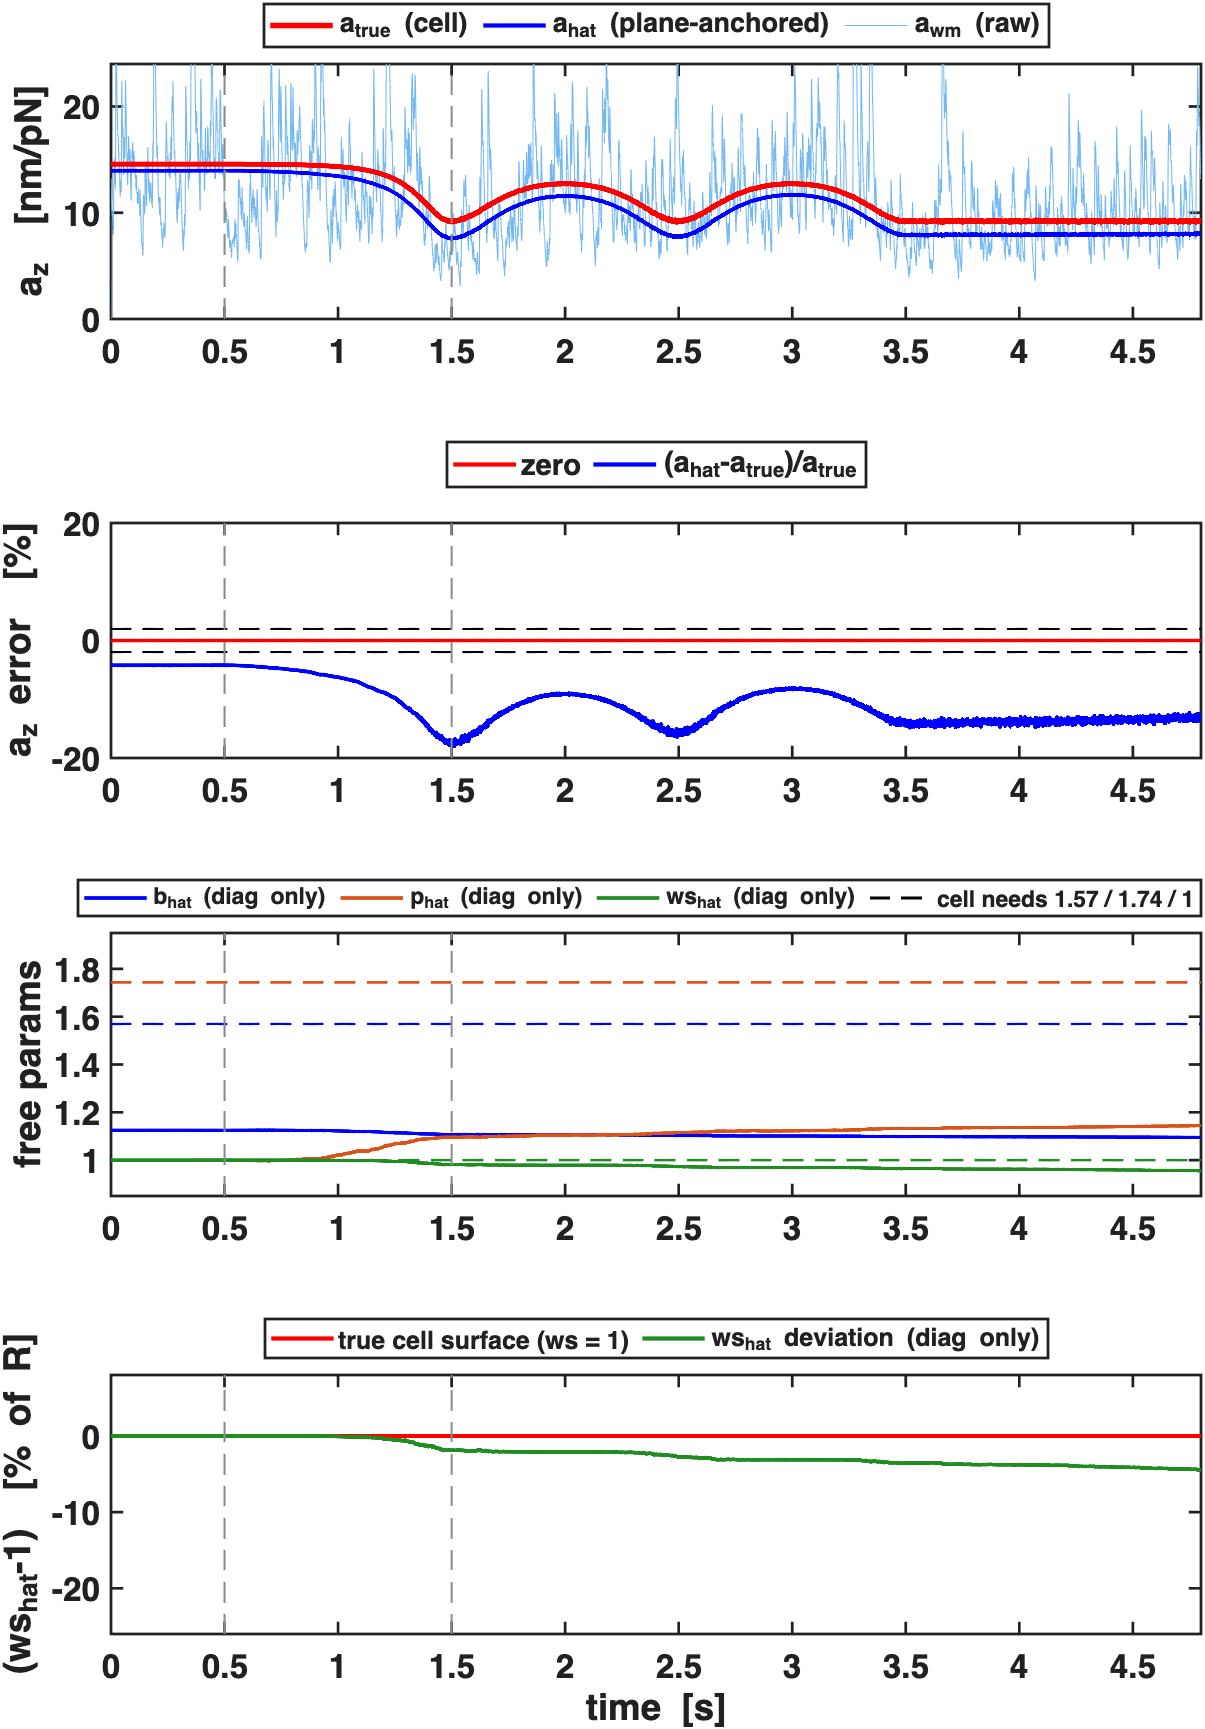
\includegraphics[width=0.49\linewidth]{figures/formB_c3_cellblind5_seed11.png}

The operating case --- same $R_c = 5\ \mu$m cell plant, but the controller
knows only the plane (anchors $9/8, 1$, priors $0.0157 / 0.0245$, origin at
the nominal contact): descent peak $19.6/17.8\,\%$, hold $-16.0/-13.6\,\%$,
$b, p$ stall near their plane anchors (final $1.10 / 1.11$ against the
$1.570 / 1.744$ the cell demands), $\hat{w}_s$ absorbs part of the mismatch by
drifting $-4.0/-4.5\,\%$, and the traversal budgets fail by $25$--$40\times$
--- a plane-anchored filter meeting a cell is wrong by $\sim\!15\,\%$ and says
so, but cannot repair itself.
\end{center}

\end{document}
